\documentclass{article}
\usepackage{ctex}
\usepackage{xeCJK}
\usepackage{fontspec}
\usepackage{amsmath}
\usepackage{graphicx}
\setmainfont{Times New Roman}
\setCJKmainfont{SimSun}

\begin{document}

\title{细菌觅食算法实例}
\author{谷超明 11731016}
\date{}
\maketitle
\tableofcontents

\section{简介}
细菌觅食算法在不同的领域中有着丰富的应用。本篇短文将从不同的方面简单介绍几种利用细菌觅食算法的实例。

\section{资源分配与调度}
利用细菌觅食算法,可以对一个需要进行大量资源分配的平台进行有效调度和动态分配。

多区域温度实验平台是对大型计算机的一个温度分配组件,通过在计算机运行的过程中根据计算量的动态变化改变工作量的资源分配。利用细菌觅食算法,可以对该温度调控平台进行动态资源划分\cite{ref1}。细菌会在整个平台表面进行随机游走,根据表面温度表示所消耗资源程度,当细菌发现更低的温度区域时,该区域可以被认为是“食物丰富”的区域,算法会要求系统对该部分区域进行资源分配,将相关的计算工作调配至该区域。从而达到对资源的高效合理应用。

该算法的工作过程大致如下:
\begin{itemize}
	\item 细菌在第一次生成时被放置在随机的搜索空间中
	\item 当前位置的资源消耗(温度)由传感器获得
	\item 一个随机翻滚将指向下一个位置
	\item 比较两个位置的资源消耗程度(温度),如果为负,则细菌将移动至新的位置,否则重新随机翻滚
\end{itemize}

从最后的结果发现,利用了细菌觅食算法的平台有更高的温度变化分布,说明更多的资源被合理分配在了不同的工作区域上,有效提高了工作效率和资源利用率。

第二个关于资源调度的实例与车间作业的调度有关。通过算法可以优化生产资源的配置。根据当前机器的空闲状态和当前工件的加工状态,选择最早可能被加工的工序来加工。在该项研究中,对细菌觅食算法进行了改进,加入了差分进化因子,增加了随机扰动,提高了细菌的搜索能力\cite{ref2}。
\vspace{1em}
\begin{center}
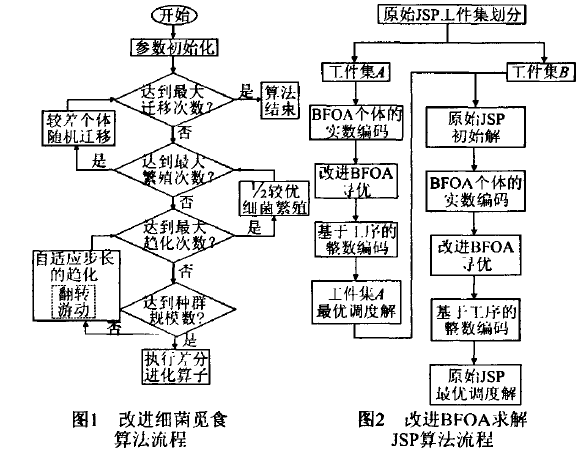
\includegraphics[scale=0.7]{flow1.png}
\end{center}
通过该算法的优化,降低了车间作业优化问题的求解难度,减少了求解时间,同时也可以得到问题的最优解。

\section{模式识别}
模式识别的一个典型应用在统计信号的独立分量分析(ICA)。利用细菌觅食算法对ICA进行分析计算,可以对其进行较好的优化。与之前常用的遗传算法GA相对比,可以发现,利用细菌觅食算法进行分析计算可以在得到相同值得情况下利用更少的估算数\cite{ref3}。如下图所示:

\begin{center}
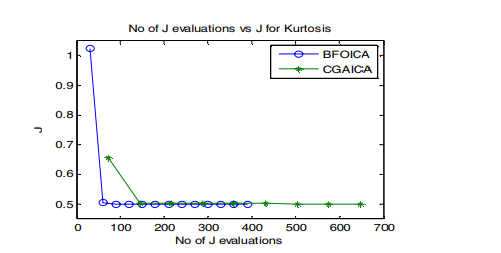
\includegraphics[scale=1]{compare.png}
\end{center}

\section{图形图像}
图形图像是计算机视觉处理的一个重要领域,其中,人脸识别是关键的技术。目前,利用人工智能算法进行人脸识别已经取得了非常重要的成果。利用细菌觅食算法,则是另一种很好的选择。在现行离散分析LDA的基础上,利用这一算法进行优化,可以取得较好的结果。细菌利用特征点作为食物进行运动,从而达到对人脸的识别处理。这一项研究与遗传算法进行了对比,在准确率上有了很大的提高\cite{ref4},如下图所示:
\begin{center}
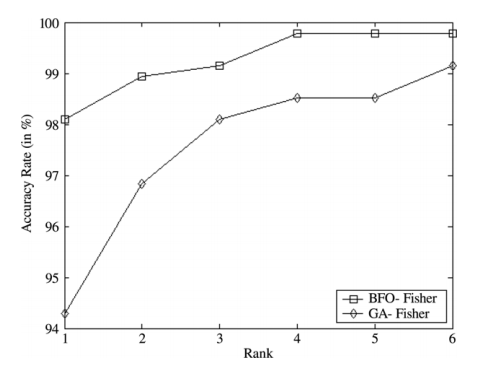
\includegraphics[scale=1]{face.png}
\end{center}

\section{算法问题}
一些在计算机领域的算法问题可以利用细菌觅食算法进行有效优化。这里以折扣背包问题为例。背包问题在资源分配,材料切割和货物装载等领域有着重要的作用。通过利用细菌觅食算法对新型背包问题的优化,并分别采用两种编码方式(二进制和四进制),可以求得近似比接近1的近似解,均为求解大规模背包问题的实用算法\cite{ref5}。基于两种编码方式的算法流程如下所示(FirBFO/SecBFO):
\begin{center}
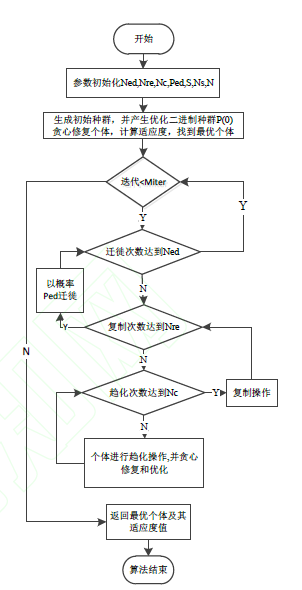
\includegraphics[scale=1]{fflow.png}
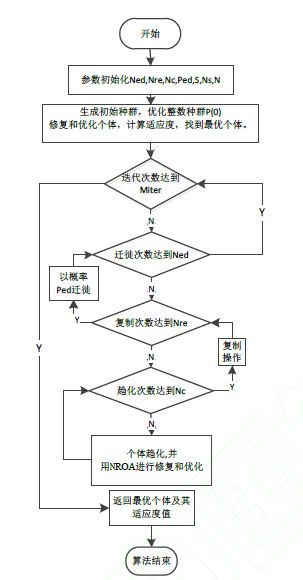
\includegraphics[scale=1]{sflow.png}
\end{center}

\vspace{2em}
细菌觅食算法还可以在其他工程问题上得到应用,例如控制预测问题等。这一算法在解决最优化问题中有着较好的性能表现,具有一定的发展潜力,可以作为特定领域的优化算法。



\begin{thebibliography}{20}
\bibitem{ref1}Munoz M A, Lopez J A, Caicedo E F. Bacteria Swarm Foraging Optimization for Dynamical Resource Allocation in a Multizone Temperature Experimentation Platform[M]// Analysis and Design of Intelligent Systems using Soft Computing Techniques. Springer Berlin Heidelberg, 2007:81-86.
\bibitem{ref2}崔静静, 孙延明, 车兰秀. 改进细菌觅食算法求解车间作业调度问题[J]. 计算机应用研究, 2011, 28(9):3324-3326.
\bibitem{ref3}Acharya D P, Panda G, Mishra S, et al. Bacteria Foraging Based Independent Component Analysis[C]// International Conference on Conference on Computational Intelligence and Multimedia Applications. IEEE, 2007:527-531.
\bibitem{ref4}Panda R, Naik M K, Panigrahi B K. Face recognition using bacterial foraging strategy[J]. Swarm \& Evolutionary Computation, 2011, 1(3):138-146.
\bibitem{ref5}刘雪静, 贺毅朝, 吴聪聪,等. 基于细菌觅食算法求解折扣\{0-1\}背包问题的研究[J]. 计算机工程与应用, 2018(2):155-162.
\end{thebibliography}

\end{document}